Feedback oppstår når output fra et system kobles tilbake på systemets input.
Det brukes til: Linearisering, stabilisering og regulering og kontroll.
Vi tegner det på følgende måte:

\begin{figure}[H]
  \caption{Negativ feedback}
  \centering
  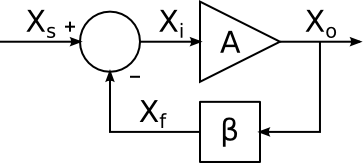
\includegraphics[width=0.67\textwidth]{./img/negfeedback}
\end{figure}

$$X_s = \text{signal inn}$$
$$X_o = \text{signal ut}$$
$$X_i = \text{signal til OpAmp}$$
$$X_f = \text{feedbacksignal}$$

Disse verdiene er gitt ved
$$X_i = X_s - \beta \cdot X_o$$
$$X_o = A \cdot (X_s - \beta \cdot X_o)
      = \frac{A \cdot X_s}{1 + A \cdot \beta}$$
$$A_f = \frac{X_o}{X_s} = \frac{A}{1 + A \cdot \beta}$$

Ved positiv feedback har vi
$$A_f = \frac{X_o}{X_s} = \frac{A}{1 - A \cdot \beta}$$
